\chapter{\textbf{Metodología}}
\label{chapter:metodologia}

\subsection*{Diagramas de bloques}
\phantomsection
\addcontentsline{toc}{section}{Diagramas de bloques}
\vspace{5mm}

\begin{itemize}
    \item \textbf{Diagrama de bloques del sistema}: es imprescindible presentar en el informe un diagrama de bloques que explique la arquitectura del sistema implementado.
    \item \textbf{Secuencia de transformación de la imagen}: será necesario realizar una secuencia en la que se muestren todas las transformaciones de la imagen (obtención de la imagen, trasnformaciones a diferentes espacios de color, máscaras, etc.).
\end{itemize}

La Figura \ref{fig:diagrama} muestra un resumen de los módulos de software que puede ayudarle a concebir su sistema.

\begin{figure}[H]
    \centering
    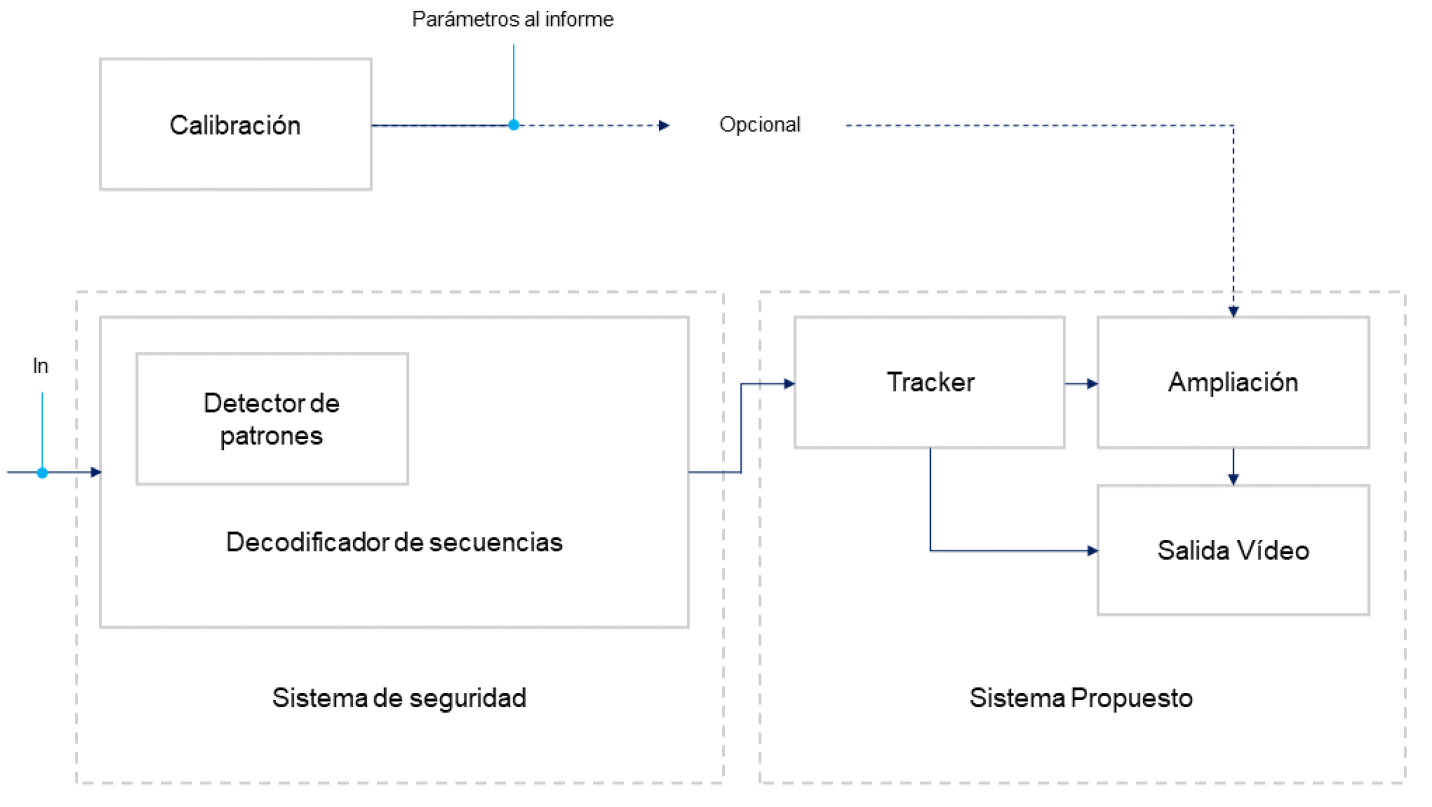
\includegraphics[width=0.85\textwidth]{Lab_Project/template/figures/diagrama.png}
    \caption{Sistema con módulos mínimos. En el módulo calibración se deberá implementar el método de calibración y el de corrección de la distorsión.}
    \label{fig:diagrama}
\end{figure}